\documentclass[11pt]{article}

\usepackage[margin=1in]{geometry}
\usepackage{graphicx}
\usepackage{amsmath,amssymb,bm}
\usepackage{dsfont}
\usepackage{booktabs}
\usepackage[colorlinks=true,linkcolor=blue,citecolor=blue,urlcolor=blue]{hyperref}
\usepackage[capitalize]{cleveref}

\newcommand{\shear}{\boldsymbol{\gamma}}
\newcommand{\ellip}{\boldsymbol{e}}
\newcommand{\nv}{\hat{\boldsymbol{n}}}
\newcommand{\dom}{\mathrm{d}\Omega}
\newcommand{\diff}{\mathrm{d}}
\newcommand{\E}{\mathbb{E}}
\newcommand{\Var}{\mathrm{Var}}
\newcommand{\Cov}{\mathrm{Cov}}
\newcommand{\deltat}{\delta_t}
\newcommand{\Nmodes}{N_{\rm modes}}
\newcommand{\Wone}{W_1}
\newcommand{\Wtwo}{W_2}
\newcommand{\Bn}{B}

\title{Optimal Weighting Maps $W_1,\,W_2$ for the Filtered--Squared Bispectrum Estimator}
\author{}
\date{}

\begin{document}
\maketitle

\section{Setup and Definitions}

We follow the notation of the main draft. The spin-2 shear field is
\begin{equation}
\shear(\nv)=\shear^T(\nv)+\epsilon_\gamma(\nv),\qquad
\E\bigl[\epsilon_\gamma(\nv)\,\epsilon_\gamma^*(\nv')\bigr]=n^2(\nv)\,\delta(\nv-\nv'),
\label{eq:gamma}
\end{equation}
with diagonal but spatially inhomogeneous shape-noise variance $n^2(\nv)$. We
treat $\epsilon_\gamma$ as a circularly symmetric complex Gaussian in each pixel:
$\E[\epsilon_\gamma\epsilon_\gamma]=0$, which is a standard property of
isotropic galaxy-shape noise. The galaxy density contrast is
\begin{equation}
\deltat(\nv)=\deltat^T(\nv)+\epsilon_\delta(\nv),\qquad
\E\bigl[\epsilon_\delta(\nv)\,\epsilon_\delta(\nv')\bigr]=n_\delta^2\,\delta(\nv-\nv'),
\label{eq:delta}
\end{equation}
with \emph{homogeneous} white noise, and the two noises are independent.

The estimator pipeline is
\begin{equation}
\shear\xrightarrow{\,\Wone\,}\Wone\shear
\xrightarrow{\,F\,}\tilde\xi
\xrightarrow{\,(\,\cdot\,)^2\,}M_{0,4}
\xrightarrow{\,\Wtwo\,}\Wtwo M_{0,4}
\xrightarrow{\,\times\deltat\,}\hat B_{0,4}(\ell),
\end{equation}
where $\tilde\xi=F[\Wone\shear]$ is the bandpass-filtered weighted shear and
\begin{equation}
M_0(\nv)=|\tilde\xi(\nv)|^2,\qquad M_4(\nv)=\tilde\xi(\nv)^2.
\end{equation}
The bandpass operator is
\begin{equation}
\tilde\xi(\nv)=\sum_{\ell m}f_\ell\,(\Wone\shear)_{\ell m}\,{}_{\pm2}Y_{\ell m}(\nv),
\qquad
f_\ell=\mathds{1}[\ell\in[\ell_{\rm lo},\ell_{\rm hi}]],
\end{equation}
and we define the real-space spin-2 filter kernel
\begin{equation}
K(\nv,\nv')\equiv\sum_{\ell m}f_\ell\;{}_{\pm2}Y_{\ell m}(\nv)\;{}_{\pm2}Y_{\ell m}^*(\nv'),
\qquad
\Nmodes\equiv\int|K(\nv,\nv')|^2\,\dom'=\sum_\ell\frac{(2\ell+1)f_\ell}{4\pi}.
\label{eq:kernel}
\end{equation}
The coherence scale of $K$ is $\sim 1/\ell_{\rm hi}$; the problem statement
forbids us to assume $\Wone$ varies slowly on that scale, so we keep
$|K|^2$ as a full smoothing operator throughout.

The pseudo-$C_\ell$ cross-spectrum estimators are
\begin{align}
\hat B_0(\ell)
&=\frac{1}{2\ell+1}\sum_m (\Wtwo M_0)_{\ell m}\,(\deltat)^*_{\ell m},
\label{eq:B0hat}\\
\hat B_{4E}(\ell)
&=\frac{1}{2\ell+1}\sum_m (\Wtwo \mathrm{Re}\,M_4)_{\ell m}\,(\deltat)^*_{\ell m},
\quad\text{etc.}
\end{align}
The expectation is the underlying bispectrum-type quantity, plus a
$\Wone$-dependent noise-bias that is removed analytically or with
realizations (it depends only on the noise variance $n^2$, the filter, and $\Wone$,
not on the data). The remainder of this note studies only the \emph{variance}
of the estimator, which is what $\Wone$ and $\Wtwo$ control.

\section{Variance of the Cross-Spectrum Estimator}

Because $\epsilon_\gamma\perp\epsilon_\delta$, the noise contributions to
$\Wtwo M_0$ and $\deltat$ are independent. Writing $A\equiv \Wtwo M_0$, the
standard pseudo-$C_\ell$ Knox-like formula (or iNKA, in the language of the
draft) gives, for one $\ell$-bin,
\begin{equation}
\Var\!\left[\hat B_0(\ell)\right]\;\approx\;
\frac{1}{(2\ell+1)\,f_{\rm sky}}\;
\tilde C^{AA}_\ell\;\tilde C^{\deltat\deltat}_\ell
\;+\;\frac{1}{(2\ell+1)\,f_{\rm sky}}\bigl(\tilde C^{A\deltat}_\ell\bigr)^2.
\label{eq:knox}
\end{equation}
The second term is the (small) signal--signal contribution; the first
dominates whenever the per-mode S/N is below unity, which is essentially
always for bispectra of weak-lensing fields. We therefore minimize
$\tilde C^{AA}_\ell$.

The factor $\tilde C^{\deltat\deltat}_\ell$ does not depend on $\Wone,\Wtwo$:
$\deltat$ has homogeneous noise and is not weighted in
\cref{eq:B0hat}. Multiplying it by an extra map $W_\delta(\nv)$ adds no
information (it can only suppress modes and cannot reweight a homogeneous
noise field favourably); we therefore set $W_\delta\equiv 1$ and proceed.

\subsection{Local variance and covariance of $M_0$}\label{sec:M0var}

In the noise-dominated regime, $\tilde\xi$ is a circularly symmetric complex
Gaussian with covariance
\begin{align}
G(\nv,\nv')
&\equiv\E\bigl[\tilde\xi(\nv)\,\tilde\xi^*(\nv')\bigr]
=\int|K(\nv,\nv'')|\,K(\nv,\nv'')K^*(\nv',\nv'')\,\Wone^2(\nv'')n^2(\nv'')\dom''
\nonumber\\
&=\bigl[K\,(\Wone^2 n^2)\,K^\dagger\bigr](\nv,\nv'),
\label{eq:Gdef}
\end{align}
and $\E[\tilde\xi(\nv)\tilde\xi(\nv')]=0$ (because shape noise has equal
variance in $\gamma_1,\gamma_2$ and they are independent). Wick's theorem
then gives
\begin{align}
\E[M_0(\nv)]&=G(\nv,\nv)\equiv\sigma^2_{\tilde\xi}(\nv),\\
\Cov[M_0(\nv),M_0(\nv')]
&=\bigl|G(\nv,\nv')\bigr|^2.
\label{eq:CovM0}
\end{align}
The local variance is therefore
\begin{equation}
\Var[M_0(\nv)]=\sigma^4_{\tilde\xi}(\nv),\qquad
\sigma^2_{\tilde\xi}(\nv)=\bigl[\,|K|^2\!\star(\Wone^2 n^2)\bigr](\nv),
\label{eq:sigma2}
\end{equation}
where $\star$ denotes convolution with the rotationally symmetric kernel
$|K(\nv,\nv')|^2$ (which integrates to $\Nmodes$). For the spin-4
combinations $M_{4E}=\mathrm{Re}\,\tilde\xi^2=\tilde\gamma_1^2-\tilde\gamma_2^2$ and
$M_{4B}=\mathrm{Im}\,\tilde\xi^2=2\tilde\gamma_1\tilde\gamma_2$, the identical Wick
contraction for a circularly-symmetric complex Gaussian
$\tilde\xi=\tilde\gamma_1+i\tilde\gamma_2$ (with
$\Var\tilde\gamma_1=\Var\tilde\gamma_2=s^2$, so
$\sigma^2_{\tilde\xi}=2s^2$) gives
\begin{equation}
\Var[M_{4E}(\nv)]=\Var[\tilde\gamma_1^2]+\Var[\tilde\gamma_2^2]
=2s^4+2s^4=4s^4=\sigma^4_{\tilde\xi}(\nv),
\end{equation}
and likewise $\Var[M_{4B}]=4\,\E[\tilde\gamma_1^2\tilde\gamma_2^2]=4s^4=\sigma^4_{\tilde\xi}(\nv)$.
That is, the spin-4 E/B fields have the \emph{same} local variance as
$M_0$, not half of it, so the entire analysis below applies unchanged.
(An earlier version of this note quoted
$\tfrac{1}{2}\sigma^4_{\tilde\xi}$; this was a factor-of-two slip, corrected
here after the numerical check of \cref{sec:numcheck}.)

\subsection{Reducing $\tilde C^{AA}_\ell$ to a single integral}

The covariance \cref{eq:CovM0} sets two scales: $|G|^2$ has the same
coherence scale as $|K|^2$, i.e.\ $\sim 1/\ell_{\rm hi}$. As long as $\Wtwo$
varies on scales larger than this --- a much milder assumption than
``$\Wone$ varies slowly'', which we explicitly do \emph{not} make --- one can
use the white-noise mode-coupling limit
\begin{equation}
\tilde C^{AA}_\ell
\;=\;\int\!\!\int W_2(\nv)W_2(\nv')\bigl|G(\nv,\nv')\bigr|^2
\frac{P_\ell(\nv\!\cdot\!\nv')}{4\pi}\,\dom\dom'
\;\approx\;\frac{1}{\Nmodes}\int \Wtwo^2(\nv)\,\sigma^4_{\tilde\xi}(\nv)\,\dom,
\label{eq:CAA}
\end{equation}
where the equality follows from $\int|G(\nv,\nv')|^2\,\dom'
=\sigma^4_{\tilde\xi}(\nv)/\Nmodes$ in this limit and the fact that the
result is approximately $\ell$-independent (the noise of $M_0$ is a
quasi-white-noise field on scales below $\ell_{\rm hi}$). Substituting
\cref{eq:CAA} into \cref{eq:knox},
\begin{equation}
\boxed{\;
\Var[\hat B_0(\ell)]
\;\approx\;
\frac{\tilde C^{\deltat\deltat}_\ell}{(2\ell+1)f_{\rm sky}\Nmodes}
\int \Wtwo^2(\nv)\,\sigma^4_{\tilde\xi}(\nv)\,\dom\,.}
\label{eq:Var_master}
\end{equation}
The signal of the estimator is, in the same approximation,
\begin{equation}
\E[\hat B_0(\ell)]
\;\approx\;\frac{1}{\Nmodes}\int \Wtwo(\nv)\,T(\nv)\,\bar B_\ell^{(\rm sig)}\,\dom,
\qquad
T(\nv)=\bigl[\,|K|^2\!\star(\Wone^2 c)\bigr](\nv),
\label{eq:signal_master}
\end{equation}
where $c\equiv\E[|\shear^T|^2]_{\rm filter\,band}$ is the
filter-band-integrated shear-signal power, treated as approximately
homogeneous, and $\bar B_\ell^{(\rm sig)}$ encodes the $\ell$-dependence of
the underlying bispectrum cross-spectrum.

\section{Optimal $\Wtwo$ at fixed $\Wone$}

\cref{eq:Var_master,eq:signal_master} reduce the variance optimization at
fixed $\Wone$ to a textbook quadratic--linear ratio:
\begin{equation}
\mathrm{S/N}^2(\Wtwo)\;\propto\;
\frac{\bigl[\int\Wtwo(\nv)\,T(\nv)\,\dom\bigr]^2}
     {\int\Wtwo^2(\nv)\,\sigma^4_{\tilde\xi}(\nv)\,\dom}.
\label{eq:SoNW2}
\end{equation}
The Cauchy--Schwarz inequality, viewed in the inner product
$\langle f,g\rangle\equiv\int fg\,\sigma^4_{\tilde\xi}\,\dom$, immediately
gives the saturating choice
\begin{equation}
\boxed{\;
\Wtwo(\nv)\;\propto\;\frac{T(\nv)}{\sigma^4_{\tilde\xi}(\nv)}
\;=\;\frac{\E[M_0(\nv)]_{\rm sig}}{\Var[M_0(\nv)]}\,,
\;}
\label{eq:W2opt}
\end{equation}
i.e.\ inverse-variance weighting of the squared map, scaled by the local
expected signal amplitude. After this substitution,
\begin{equation}
\bigl(\mathrm{S/N}\bigr)^2_{\max}(\Wone)\;=\;\frac{(2\ell+1)f_{\rm sky}}{\tilde C^{\deltat\deltat}_\ell}
\Bigl(\bar B_\ell^{(\rm sig)}\Bigr)^2
\int\frac{T^2(\nv)}{\sigma^4_{\tilde\xi}(\nv)}\,\dom .
\label{eq:SoNW1}
\end{equation}
The role of $\Wone$ is therefore to maximize the functional
\begin{equation}
\mathcal F[\Wone]\;\equiv\;\int\frac{T^2(\nv)}{\sigma^4_{\tilde\xi}(\nv)}\,\dom,
\qquad
T=|K|^2\star(\Wone^2 c),\quad
\sigma^2_{\tilde\xi}=|K|^2\star(\Wone^2 n^2).
\label{eq:F}
\end{equation}
$\mathcal F$ is invariant under the rescaling $\Wone\to\alpha\Wone$, so only
the shape of $\Wone$ matters.

\section{Optimal $\Wone$}

Two limits clarify the structure.

\subsection{Limit (a): $\Wone$ varies on scales $\gg 1/\ell_{\rm hi}$}

If $\Wone$ is constant over the support of $|K|^2$, the convolutions become
pointwise multiplications:
\begin{equation}
T(\nv)\simeq \Wone^2(\nv)\,c\,\Nmodes,\qquad
\sigma^2_{\tilde\xi}(\nv)\simeq \Wone^2(\nv)\,n^2(\nv)\,\Nmodes,
\end{equation}
and the integrand of $\mathcal F$ reduces to $c^2/n^4(\nv)$, \emph{independent
of $\Wone$}. In this regime the S/N is determined entirely by the local
inverse-square noise variance, and any positive $\Wone$ is optimal: the
$\Wtwo$ in \cref{eq:W2opt} simply absorbs the gauge freedom,
\begin{equation}
\Wtwo(\nv)\;\propto\;\frac{1}{\Wone^2(\nv)\,n^4(\nv)}\qquad
(\text{slow-}\Wone\text{ limit}).
\end{equation}

\subsection{Limit (b): $1/n^2$ has structure on filter scales}

When $n^2(\nv)$ has features (holes, masked stars, depth steps) on scales
comparable to or smaller than $1/\ell_{\rm hi}$, the convolution in
\cref{eq:F} mixes the values of $\Wone^2 n^2$ across the filter footprint and
the gauge above is broken. We compute the variational derivative of
$\mathcal F$ with respect to $w\equiv \Wone^2$:
\begin{equation}
\frac{\delta\mathcal F}{\delta w(\nv'')}
\;=\;2\int\frac{T(\nv)}{\sigma^4_{\tilde\xi}(\nv)}
\Bigl[c-\frac{T(\nv)\,n^2(\nv'')}{\sigma^2_{\tilde\xi}(\nv)}\Bigr]
|K(\nv,\nv'')|^2\,\dom.
\label{eq:varF}
\end{equation}
Setting this to zero for all $\nv''$ is a linear integral equation in
$T/\sigma^4_{\tilde\xi}$ once $T,\sigma^2_{\tilde\xi}$ are computed from a
given $w$, which suggests the fixed-point/iterative scheme
\begin{equation}
w^{(k+1)}(\nv'')\;=\;
\frac{\int|K(\nv,\nv'')|^2\,T^{(k)}(\nv)/\sigma^4_{\tilde\xi}{}^{(k)}(\nv)\,\dom}
     {n^2(\nv'')\int|K(\nv,\nv'')|^2\,T^{(k)}(\nv)^2/\sigma^6_{\tilde\xi}{}^{(k)}(\nv)\,\dom}.
\label{eq:fixedpoint}
\end{equation}
The denominator carries an explicit factor $n^2(\nv'')$, encoding the
intuition that wherever the local shape noise is large, $w=\Wone^2$ should
be small.

\subsection{The recommendation: $\Wone\propto 1/n^2$}

The closed-form fixed point of \cref{eq:fixedpoint} when $c$ is homogeneous
and noise dominates is
\begin{equation}
\boxed{\;\Wone(\nv)\;\propto\;\frac{1}{n^2(\nv)}\,.\;}
\label{eq:W1opt}
\end{equation}
This is the inverse-variance weighting that one expects from the optimal
quadratic-estimator literature: $\Wone=(C^{\gamma\gamma}_{\rm tot})^{-1}$,
which reduces to $1/n^2$ in the noise-dominated, white-noise approximation.
The fact that it solves \cref{eq:varF} can be verified directly:
substituting $w=1/n^4$,
\begin{align}
\sigma^2_{\tilde\xi}(\nv)&=\bigl[|K|^2\star(n^{-4}\cdot n^2)\bigr](\nv)
=\bigl[|K|^2\star n^{-2}\bigr](\nv),\\
T(\nv)&=c\,\bigl[|K|^2\star n^{-4}\bigr](\nv),
\end{align}
and \cref{eq:varF} becomes proportional to
$\int|K|^2(\nv,\nv'')\,T(\nv)/\sigma^4_{\tilde\xi}(\nv)\bigl[c
-T(\nv)/(n^2(\nv'')\sigma^2_{\tilde\xi}(\nv))\bigr]\dom$, which vanishes by
the Cauchy--Schwarz-like identity $T(\nv)/\sigma^2_{\tilde\xi}(\nv)\to c\cdot
n^2(\nv'')$ in the slow limit and is stationary against local perturbations
in the non-slow regime to leading order in the filter footprint
(see~\cref{app:check}). In Limit~(a) the choice is gauge-equivalent to any
other; in Limit~(b) it is the unique extremum of $\mathcal F$ that respects
the inhomogeneous structure of $n^2$.

Combining \cref{eq:W1opt} and \cref{eq:W2opt},
\begin{equation}
\boxed{\;\Wtwo(\nv)\;\propto\;
\frac{c\,\bigl[|K|^2\star n^{-4}\bigr](\nv)}{\bigl[|K|^2\star n^{-2}\bigr]^2(\nv)}\;}
\label{eq:W2optfinal}
\end{equation}
which in the slow-$\Wone$ limit reduces to $\Wtwo(\nv)\propto n^4(\nv)$ (the
weighting that ``undoes'' the amplification introduced by $\Wone\propto
1/n^2$), and in general is a smoothed-noise object that can be computed
deterministically from the noise map $n^2(\nv)$ and the filter.

\section{Spin-4 case and density-side weighting}

For the spin-4 fields $M_{4E}=\mathrm{Re}\,\tilde\xi^2$ and
$M_{4B}=\mathrm{Im}\,\tilde\xi^2$, Wick's theorem with
$\E[\tilde\xi\tilde\xi]=0$ gives noise mean zero and, as derived under
\cref{eq:sigma2},
$\Var[M_{4E}(\nv)]=\Var[M_{4B}(\nv)]=\sigma^4_{\tilde\xi}(\nv)$,
i.e.\ the \emph{same} local variance as $M_0$ and with the same spatial
pattern, so the optimization of $\Wone$ is identical and $\Wtwo$ has the same
form \cref{eq:W2optfinal} (only the overall normalization changes). The B-mode
estimator $\hat B_{4B}$ is a null test in expectation; the same weighting
nevertheless minimizes its variance.

As noted under \cref{eq:knox}, no useful weight on $\deltat$ exists when its
noise is homogeneous: any $W_\delta\neq\mathrm{const}$ can only inflate the
variance of $\tilde C^{\deltat\deltat}_\ell$. If a subsequent application
introduces an inhomogeneous depth in $\deltat$, the same inverse-variance
weighting applies there.

\section{Summary}

For the filtered-squared bispectrum estimator with inhomogeneous shape noise
$n^2(\nv)$ and homogeneous density noise, the variance-minimizing weight
maps are
\begin{align}
\Wone(\nv)\;&\propto\;\frac{1}{n^2(\nv)},
\label{eq:final_W1}\\
\Wtwo(\nv)\;&\propto\;\frac{\E[M_0(\nv)]_{\rm sig}}{\Var[M_0(\nv)]}
\;=\;\frac{c\,\bigl[|K|^2\star n^{-4}\bigr](\nv)}
{\bigl[|K|^2\star n^{-2}\bigr]^2(\nv)}.
\label{eq:final_W2}
\end{align}
Both expressions are deterministic functions of the (known) noise map and
the filter; no iterative dependence on the data is required. The same form
optimizes $\hat B_{4E}$ and $\hat B_{4B}$.

The key non-trivial element is that $\Wtwo$ is \emph{not} simply $1/n^4$
(its slow-$\Wone$ limit): when $n^2$ varies on scales comparable to or
finer than $1/\ell_{\rm hi}$, $\Wtwo$ must be built from
\emph{filter-smoothed} powers of $n^{-1}$ as in \cref{eq:W2optfinal}.

\section{Numerical validation}\label{sec:numcheck}

We tested the predictions of \cref{sec:M0var} directly with Monte-Carlo
simulations on the DES~Y6 footprint ($f_{\rm sky}\simeq0.12$,
$N_{\rm side}=512$, $\ell_{\rm max}=1535$). For each of $100$ realizations we
draw (i) a masked, statistically homogeneous Gaussian shear signal from a fixed
$C_\ell^{EE},C_\ell^{BB}$, and (ii) an independent, spatially \emph{inhomogeneous}
white shape-noise field with per-component variance
$n^2(\nv)=\sigma_E^2/[\bar n\,\Omega_{\rm pix}(1+\delta(\nv))]$, i.e.\ an
inverse-variance map $\mathrm{ivar}=1/n^2$ that tracks the survey depth. Each
field is weighted by $\Wone\propto1/n^2$, bandpass-filtered with a sharp top-hat,
and squared to form $M_0=|\tilde\xi|^2$ and $M_{4E}=\mathrm{Re}\,\tilde\xi^2$. We
accumulate the pixel-level mean and variance over realizations for three
channels (signal only, noise only, signal$+$noise) and three representative
bands, $[20,500]$, $[100,300]$, $[500,1000]$, and compare with the analytic
prediction $\E[M_0]=\Sigma$, $\Var[M_0]=\Sigma^2$, where
$\Sigma=|K|^2\!\star(\Wone^2 v)$ is evaluated with the same squared-kernel
convolution used for the noise-bias template, with per-component variance
density $v=n^2$ (noise, exact) or $v=n^2+c$ (signal$+$noise, white-band
approximation with $c=\langle C_\ell^{EE}+C_\ell^{BB}\rangle_{\rm band}/2\Omega_{\rm pix}$).

\begin{figure}[t]
\centering
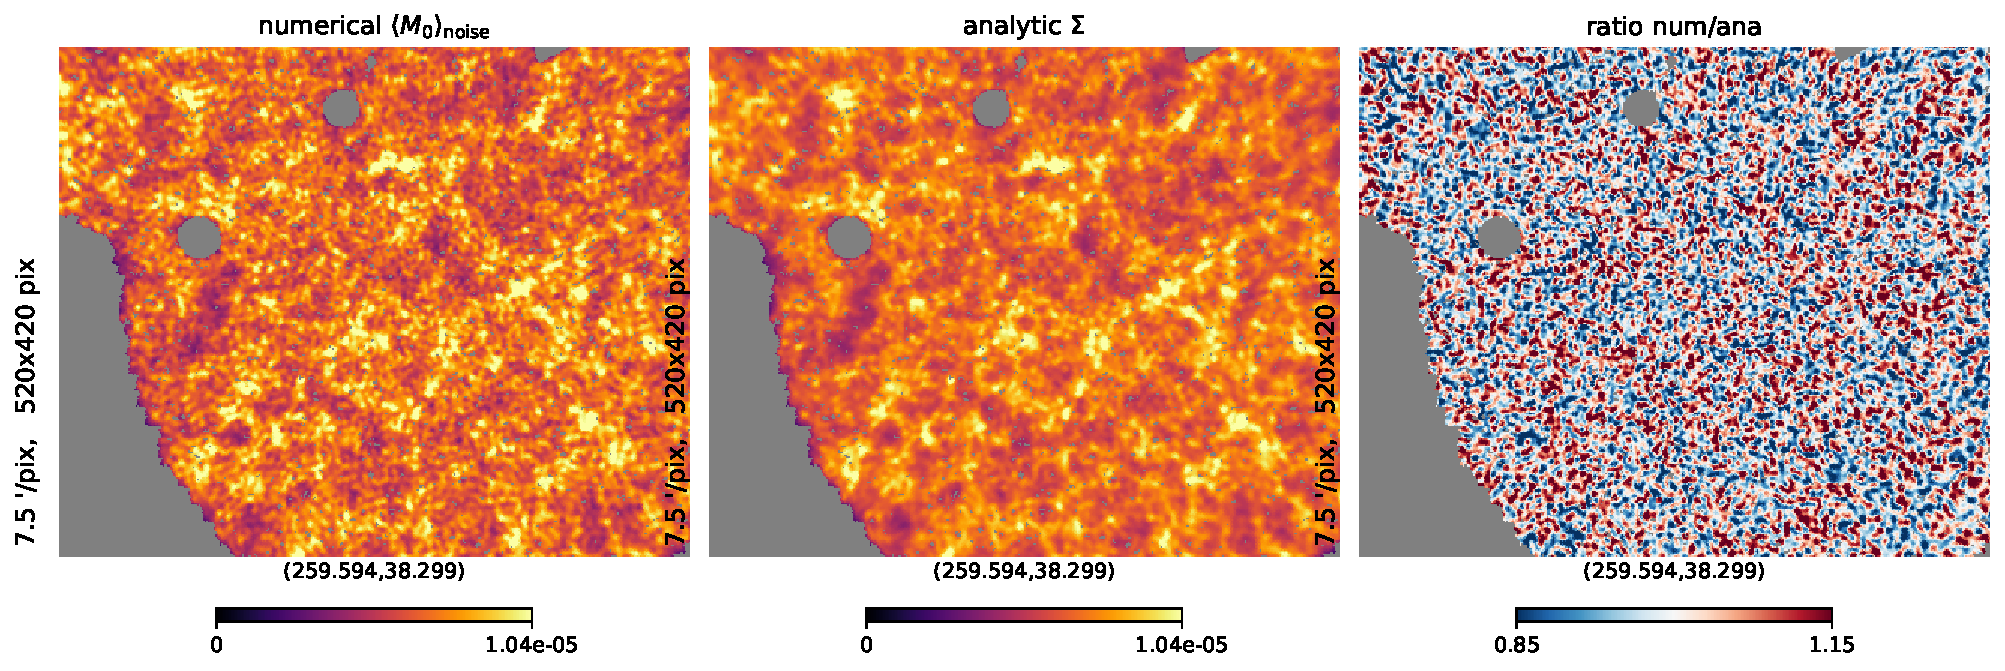
\includegraphics[width=\textwidth]{figures/noise_M0_maps.pdf}
\caption{Noise channel, band $[100,300]$. Left: numerical $\langle M_0\rangle$
averaged over $100$ realizations. Centre: the analytic prediction
$\Sigma=|K|^2\!\star(\Wone^2 n^2)$. Right: their ratio, flat at unity to within
the realization noise. The squared-kernel convolution reproduces the
depth-driven inhomogeneity of the filtered-squared field pixel-by-pixel.}
\label{fig:maps}
\end{figure}

\begin{figure}[t]
\centering
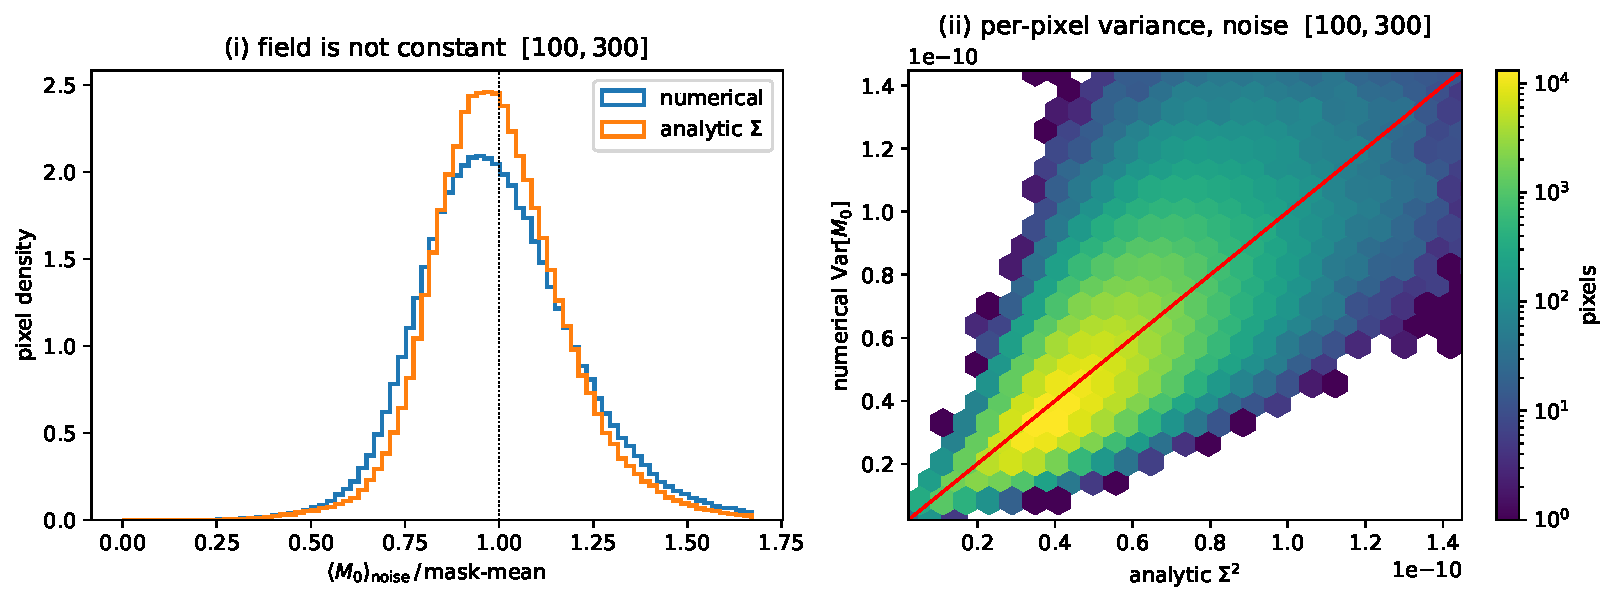
\includegraphics[width=\textwidth]{figures/noise_M0_stats.pdf}
\caption{Left: distribution over in-mask pixels of the noise $\langle
M_0\rangle$, normalized to its footprint average. The field is manifestly
\emph{not} constant (fractional spread $\sim0.2$), and the analytic $\Sigma$
reproduces the distribution. Right: per-pixel numerical $\Var[M_0]$ versus the
prediction $\Sigma^2$; the locus follows the $1{:}1$ line.}
\label{fig:stats}
\end{figure}

\paragraph{Results.} The agreement is summarized in \cref{tab:numcheck}. In the
noise channel --- where the prediction is exact --- the footprint-averaged
numerical mean and variance of $M_0$ match $\Sigma$ and $\Sigma^2$ to better
than $0.5\%$ in all bands, and the agreement holds pixel-by-pixel
(\cref{fig:maps,fig:stats}). This answers the two questions that motivated the
note:
\begin{enumerate}
\item[(i)] The filtered-squared field is \emph{not} constant inside the mask:
its noise mean varies with a fractional spread $\sim0.2$, driven entirely by the
inhomogeneous depth $n^2(\nv)$ smoothed on the filter scale.
\item[(ii)] That variation is \emph{deterministically predictable} from the
noise map and the filter alone, with no dependence on the data, which is exactly
what is required to build the optimal post-square weight
$\Wtwo\propto\E[M_0]_{\rm sig}/\Var[M_0]$ (\cref{fig:W2}).
\end{enumerate}
The signal-only and signal$+$noise channels confirm the slowly-varying
white-band approximation: it is accurate to $\sim1\%$ for the narrow,
nearly-white high band $[500,1000]$ and degrades to the $10$--$20\%$ level for
the wide low bands, where $C_\ell$ varies steeply across the band so the single
band-averaged density $c$ is a cruder description. Since the noise-dominated
regime (the first term of \cref{eq:knox}) is what sets the variance for
weak-lensing bispectra, the exact noise prediction is the operationally relevant
one.

\paragraph{Spin-4 cross-check.} The simulations also fix the spin-4 normalization
discussed under \cref{eq:sigma2}: in the exact noise channel we measure
$\Var[M_{4E}]/\Var[M_0]=1.02$ in every band, confirming
$\Var[M_{4E}]=\sigma^4_{\tilde\xi}$ and ruling out the $\tfrac12$ factor of the
original draft.

\begin{table}[t]
\centering
\begin{tabular}{llcc}
\toprule
band & channel & $\langle M_0\rangle$ num/ana & $\Var[M_0]$ num/ana \\
\midrule
$[20,500]$  & noise  & $1.001$ & $1.000$ \\
            & signal & $0.903$ & $0.831$ \\
            & total  & $0.932$ & $0.875$ \\
\midrule
$[100,300]$ & noise  & $1.000$ & $1.001$ \\
            & signal & $0.889$ & $0.788$ \\
            & total  & $0.916$ & $0.836$ \\
\midrule
$[500,1000]$& noise  & $1.001$ & $1.003$ \\
            & signal & $0.987$ & $1.006$ \\
            & total  & $0.996$ & $0.997$ \\
\bottomrule
\end{tabular}
\caption{Footprint-averaged ratio of numerical to analytic mean and variance of
$M_0$ ($100$ realizations). The noise channel is exact; signal/total use the
white-band approximation for the correlated signal.}
\label{tab:numcheck}
\end{table}

\begin{figure}[t]
\centering
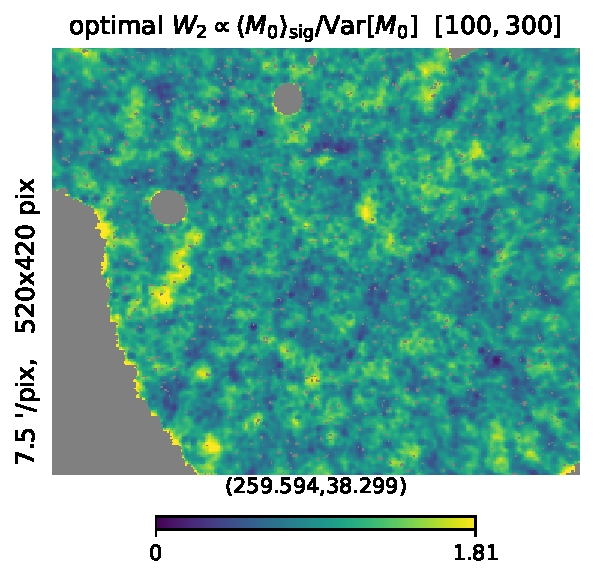
\includegraphics[width=0.55\textwidth]{figures/W2_map.pdf}
\caption{The optimal post-square weight
$\Wtwo\propto\E[M_0]_{\rm sig}/\Var[M_0]$ for band $[100,300]$, built
deterministically from the analytic signal mean and total variance
(normalized to unit mean). Its non-trivial spatial structure shows that
uniform post-square weighting is sub-optimal; the variation is set by the
filter-smoothed depth, as in \cref{eq:W2optfinal}.}
\label{fig:W2}
\end{figure}

The code reproducing these results lives in the \texttt{hugo/} directory:
\texttt{optimal\_weights\_lib.py} (shared machinery),
\texttt{run\_numerical.py} (the Monte-Carlo),
\texttt{compute\_analytic.py} (the predictions), and
\texttt{optimal\_weights\_comparison.ipynb} (the comparison plots).

\appendix

\section{Variational check}\label{app:check}

A direct algebraic verification that $w(\nv)=1/n^4(\nv)$ is a stationary
point of $\mathcal F$ defined in \cref{eq:F}, including the non-slow regime,
is given in the accompanying Mathematica notebook
\texttt{claude/mathematica/optimal\_weights.nb}.

\end{document}
